\chapter{实验结果与分析}
\label {exp}
本章主要介绍如何对本文中所提出的补丁兼容性检测方法的工具实现进行实验,并且给出了实验结果和分析。

\section{实验设计}
\label {exp_des}

考虑到本文中所要讨论的软件补丁兼容性检测问题,这是一个工业界中常见的实际问题,广泛存在于各类项目中。考虑到工业界中的实际情况,本文中在对该检测工具进行实验时,应当选择工业界中常见、常用的中大型项目。如此一来,实验的结果就可以具有较强的说服力,能够回答本文中所提出的方法是否能够切实解决工业生产中面对的实际问题。

可见,实验应当回答如下的问题:
\begin{itemize}
	\item 检测工具是否能够成功对实际项目进行分析?该项可以说明本文方法的可用性。
	\item 检测工具是否能够找到补丁的兼容性问题?找到的冲突是否存在误报的情况?该项可以说明本文方法的正确性。
	\item 检测工具能找到的兼容性问题有多少?该项可以说明本文方法的实用性。
\end{itemize}

因此,本章中应当对这些问题给予回答,并给出相应的量化表述。

根据上面的需求,本章中的实验过程可以设计如图\ref {des_exp}所示。

\begin{figure}[H]
	\centering
	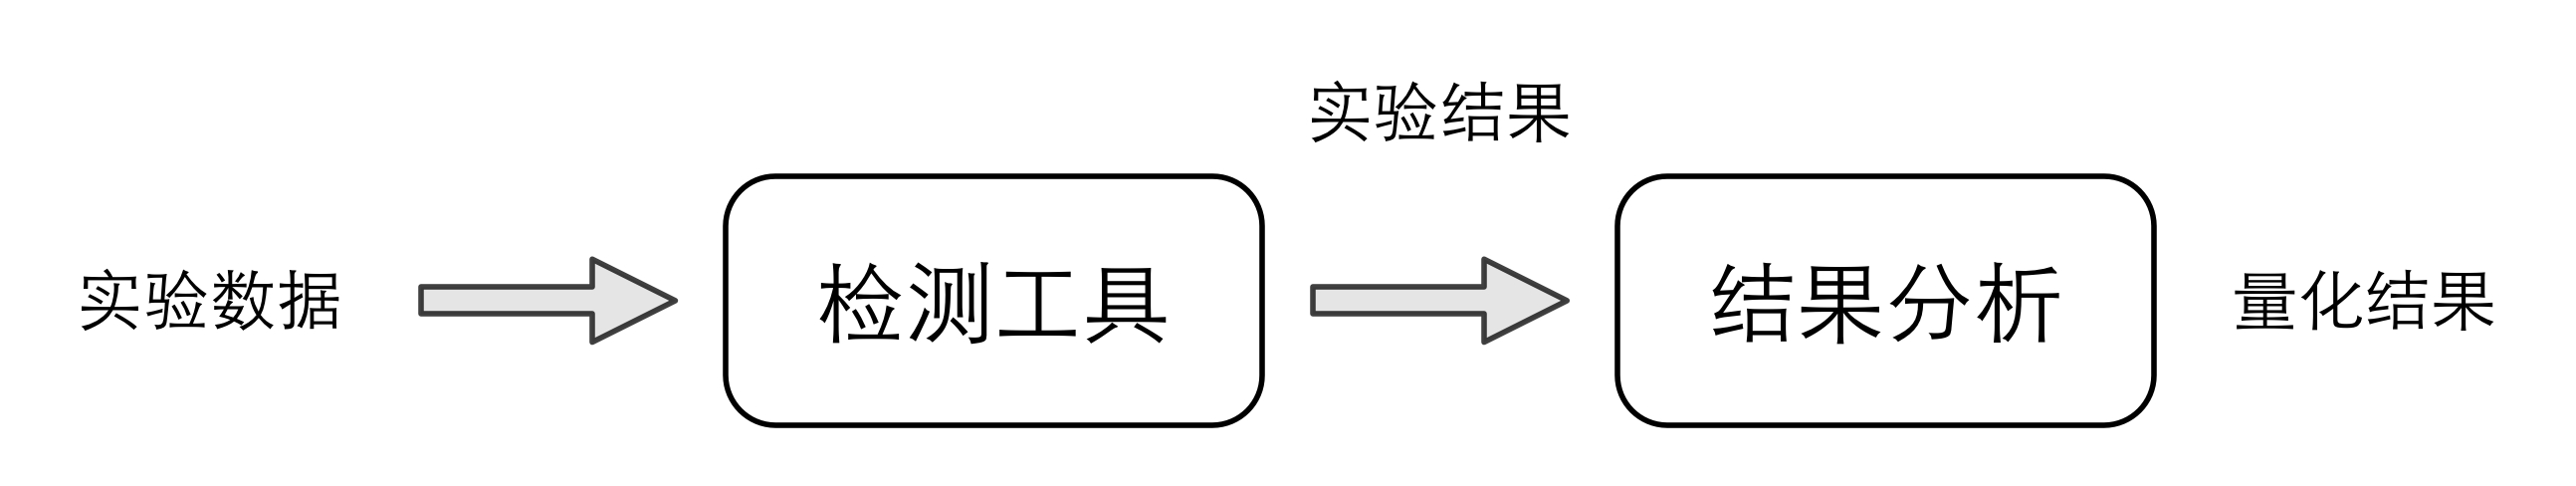
\includegraphics[width=.8\columnwidth]{chap07_exp}
	\caption {实验设计}
	\label {des_exp}	
\end{figure}


下面就本文中所采用的实验平台,对其配置说明如下:
\begin{itemize}
	\item 操作系统:Mac OS X 10.9
	\item CPU:2.4 GHz Intel Core i5
	\item 内存:8 GB 1600 MHz DDR3
	\item 硬盘:251 GB APPLE SSD SM0256F Media
\end{itemize}

\section{实验案例}
\label {exp_data}

为了使实验结果更具有说服力,本文在实验案例的选择中考虑采用工业界中的实际项目来进行实验,以测试检测工具的可靠性和可用性。

因此,本文中将采用Eclipse JDT Core项目作为实验案例。JDT Core是Eclipse工具的Java基础组件,它主要提供了如下功能:
\begin{itemize}
	\item Java编译器。
	\item Java文档模型。
	\item Java模型。
	\item 编程帮助。
	\item 搜索。
	\item 源代码排版。
\end{itemize}

该项目的相关信息可以参见表\ref {jdt_core}。

\begin{table}[H]
	\caption{Eclipse JDT Core}
	\label{jdt_core}
	\centering
	\begin{tabular}{llc}
		\toprule[1.5pt]
		{\heiti 信息} & {\heiti 描述} \\\midrule[1pt]
		语言 & Java \\
		文件数 & 约1100个\\
		代码量 & 约3W行\\
		\bottomrule[1.5pt]
	\end{tabular}
\end{table}

Groovy-Eclipse是一个Eclipse的插件集合,用于为Groovy项目提供Eclipse的工具支持。Groovy是一门类似于Java的面向对象编程语言,Groovy代码可以被编译器转化为Java字节码,从而在JVM上运行。由于这一特性,使得Groovy可以调用其他Java语言编写的库,从而大大丰富了其可用性。

Groovy-Eclipse中提供了一个补丁后的JDT Core版本,该补丁主要用于增强JDT Core的功能,使其能够无缝编译Groovy代码。因而我们选择了该补丁作为实验数据中逻辑版本$v_3$的来源。

JDT Core项目截止目前已推出发行版4.4.2,我们从中选择了若干个发行版作为实验数据中逻辑版本$v_1$和$v_2$的来源。逻辑版本的具体说明可以参考表\ref {exp_version},具体的实验数据选择可以参考表\ref {exp_data},其中由于逻辑版本$v_4$由版本合并而来,因此在表\ref {exp_data}中不予列出。

从表\ref {exp_data}中可见,我们一共选择了7个发行版本作为逻辑版本$v_2$的来源。也就是说,我们将以固定的逻辑版本$v_1$和$v_3$为基准,并选择不断变化的逻辑版本$v_2$来进行实验。

这样做的好处是我们可以更加清晰的了解本文中所提出的补丁兼容性分析方法,包括:
\begin{itemize}
	\item 是否可针对工业界实际项目进行分析?
	\item 是否切实贴合工业界的实际需求?
	\item 是否对同一软件系统的多个不同版本具有普遍适用性?
\end{itemize}

\begin{table}
	\caption{实验数据}
	\label{exp_data}
	\centering
	\begin{tabular}{llc}
		\toprule[1.5pt]
		{\heiti 代码} & {\heiti 发行版本} & {\heiti 逻辑版本} \\\midrule[1pt]
		Eclipse JDT Core & 4.3.2 & $v_1$ \\
		Groovy-Eclipse JDT Core & 4.3.2 & $v_3$\\
		Eclipse JDT Core & 4.4 & $v_2$\\
		Eclipse JDT Core & 4.4.2 & $v_2$\\
		Eclipse JDT Core & 4.3 & $v_2$\\
		Eclipse JDT Core & 4.3.1 & $v_2$\\
		Eclipse JDT Core & 4.2 & $v_2$\\
		Eclipse JDT Core & 4.2.1 & $v_2$\\
		Eclipse JDT Core & 4.2.2 & $v_2$\\
		\bottomrule[1.5pt]
	\end{tabular}
\end{table}

\begin{table}
	\caption{逻辑版本对照表}
	\label{exp_version}
	\centering
	\begin{tabular}{llc}
		\toprule[1.5pt]
		{\heiti 逻辑版本} & {\heiti 描述} \\\midrule[1pt]
		$v_1$ & 旧版本 \\
		$v_2$ & 新版本\\
		$v_3$ & 应用补丁$p_1$后旧版本\\
		$v_4$ & 版本$v_2$和版本$v_3$合并后版本,相当于应用补丁$p_1$后新版本\\
		\bottomrule[1.5pt]
	\end{tabular}
\end{table}

\section{实验结果与分析}
\label {exp_result}

由于检测工具由多个模块构成,因此实验是分步进行的,本节中给出每个模块的输入输出数据,并对其结果加以分析。
\subsection{版本迁移模块}

根据我们所选择的实验案例,其所有版本的提交与合并过程可以参考图\ref {exp_git_merge}。

可见,该过程中我们以Eclipse JDT Core发行版4.3.2作为旧版本$v_1$,以Groovy-Eclipse JDT Core发行版4.3.2作为版本$v_3$,以其他Eclipse JDT 发行版作为版本$v_2$,并为不同的版本$v_2$创建了独立分支,用于各自实现版本合并过程。


在版本合并的过程中,我们检测到的待解决冲突数量可以参见表\ref {data_git_merge}。通过Beyond Compare工具,这些冲突都能够得到解决。
可以发现,冲突最少的是版本4.3.x,这可能是由于版本4.3到版本4.3.2的升级过程改动较少而造成的。而对于版本4.4.x来说,冲突数量陡增,这可能是由于版本升级较大的缘故。
%根据实验结果,这些冲突95\%以上都可以采用Beyond Compare工具中推荐的方案进行解决,只有极少部分代码需要进行手工解决。

\begin{table}
	\caption{版本合并结果结果}
	\label{data_git_merge}
	\centering
	\begin{tabular}{llcc}
		\toprule[1.5pt]
		{\heiti 代码} & {\heiti 发行版本} & {\heiti 冲突文件数量} & {\heiti 所有文件}\\\midrule[1pt]
		Eclipse JDT Core & 4.4 & 313 & 1285\\
		Eclipse JDT Core & 4.4.2 & 596 & 1281\\
		Eclipse JDT Core & 4.3 & 10 & 1209\\
		Eclipse JDT Core & 4.3.1 & 10 & 1209\\
		Eclipse JDT Core & 4.2 & 50 & 1205\\
		Eclipse JDT Core & 4.2.1 & 49 & 1205\\
		Eclipse JDT Core & 4.2.2 & 49 & 1205\\
		\bottomrule[1.5pt]
	\end{tabular}
\end{table}


\begin{figure}[H]
	\centering
	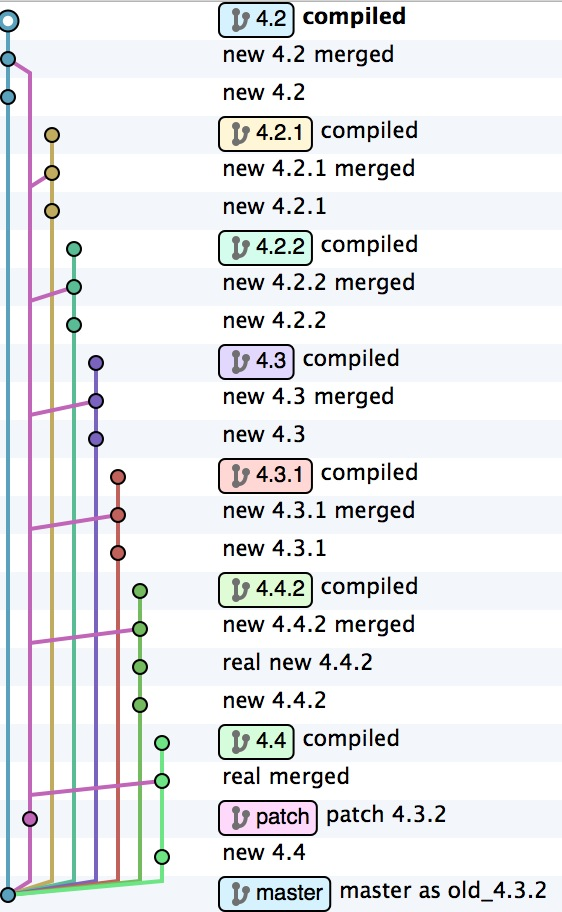
\includegraphics[height=.8\columnwidth]{chap07_git_merge}
	\caption {git版本合并}
	\label {exp_git_merge}	
\end{figure}

在实际操作过程中,由于后续的影响域分析模块需要提供Java代码编译后产生的Class文件,我们对于合并后的版本$v_4$还需要进行编译。实验过程中,绝大多数的文件都能够正常编译通过,只有极少部分文件由于合并出错等原因而无法编译通过。该部分数据可以参考表\ref {data_git_merge2}。对比编译过程中的错误数据与版本合并中的冲突数据,可见二者的变化过程是较为吻合的。

\begin{table}
	\caption{编译结果}
	\label{data_git_merge2}
	\centering
	\begin{tabular}{llcc}
		\toprule[1.5pt]
		{\heiti 代码} & {\heiti 发行版本} & {\heiti 编译失败文件} & {\heiti 所有文件}\\\midrule[1pt]
		Eclipse JDT Core & 4.4 & 23 & 1285\\
		Eclipse JDT Core & 4.4.2 & 18 & 1281\\
		Eclipse JDT Core & 4.3 & 0 & 1209\\
		Eclipse JDT Core & 4.3.1 & 1 & 1209\\
		Eclipse JDT Core & 4.2 & 4 & 1205\\
		Eclipse JDT Core & 4.2.1 & 4 & 1205\\
		Eclipse JDT Core & 4.2.2 & 1 & 1205\\
		\bottomrule[1.5pt]
	\end{tabular}
\end{table}

如上所述,我们的版本迁移模块是可用且有效的。

%在实际执行过程中,需要解决的版本合并冲突可能非常多,由于git在引导第三方工具进行冲突解决时采用的是交互式的策略,因而冲突解决需要花费较长时间和较多人力资源。为此本文采用了Apple Script撰写的脚本来辅助完成这个过程,尽可能的将其自动化。
%
%由于大部分情况下Beyond Compare提供的解决方案都是可行的,因而我们只需要采纳该解决方案即可,如果该工具无法直接提供完全正确的解决方案,则再进行人工解决即可。因而该脚本主要用于自动化实现与图形化GUI工具的交互过程,如下所述。
%
%\begin{lstlisting} [style=BashInputStyle]
%tell application "System Events"
%	repeat 300 times
%		delay 1
%		set theName to name of the first process
%			whose frontmost is true	
%		if theName is "BCompare" then		
%			delay 1	
%			keystroke "s" using {command down}	
%			delay 1	
%			if theName is "BCompare" then
%				keystroke "w" using {command down}
%			end if		
%			delay 1		
%		else
%			delay 1
%		end if
%	end repeat
%end tell
%\end{lstlisting}

\subsection{影响域分析模块}

由于整个影响域分析模块可以分为差异性分析模块和影响分析模块两个子模块,下面将分别阐述这两个子模块的实验结果并对其结果进行分析。

\subsubsection{差异性分析模块}

在差异性分析模块中,我们比较关注预处理算法的结果以及能够成功完成差异性分析的文件数量。

对于预处理算法而言,实验结果如表\ref {data_differ_1}所示。

\begin{table}[H]
	\caption{Program Differ结果}
	\label{data_differ_1}
	\centering
	\begin{tabular}{llccc}
		\toprule[1.5pt]
		{\heiti 代码} & {\heiti 发行版本} & {\heiti 预处理数} & {\heiti $diff(v_2,v_1)$文件数} & {\heiti $diff(v_2,v_4)$文件数} \\\midrule[1pt]
		Eclipse JDT Core & 4.4	& 91 & 1088 & 1172	\\		
		Eclipse JDT Core & 4.4.2 & 94 & 1097 & 1178		\\
		Eclipse JDT Core & 4.3 	& 110 & 1126 & 1124			\\
		Eclipse JDT Core & 4.3.1 & 110 & 1126 & 1123			\\
		Eclipse JDT Core & 4.2 	& 99 & 1115 & 1117		\\
		Eclipse JDT Core & 4.2.1 & 99 & 1115 & 1116			\\
		Eclipse JDT Core & 4.2.2 & 99 & 1115 & 1116		\\
		\bottomrule[1.5pt]
	\end{tabular}
\end{table}

可见,我们的预处理算法对原有的ASTro工具的直接输出结果进行了有效的过滤。预处理算法的好处在之后的影响分析模块中体现得更为明显。

整个差异性分析模块的输出结果如表\ref {data_differ_2}和表\ref {data_differ_3}所述。

\begin{table}[H]
	\caption{Program Differ结果}
	\label{data_differ_2}
	\centering
	\begin{tabular}{llccc}
		\toprule[1.5pt]
		{\heiti $v_1$} & {\heiti $v_2$} & {\heiti $diff(v_2,v_1)$文件数} & {\heiti $v_2$文件} & {\heiti $v_1$文件} \\\midrule[1pt]
		4.3.2 & 4.4	& 1088 & 1272 & 1200\\		
		4.3.2 & 4.4.2 & 1097 & 1272	& 1200	\\
		4.3.2 & 4.3 	 & 1126 & 1200	& 1200		\\
		4.3.2 & 4.3.1  & 1126 & 1200 & 1200			\\
		4.3.2 & 4.2 	& 1115 & 1196 & 1200		\\
		4.3.2 & 4.2.1 & 1115 & 1196 & 1200		\\
		4.3.2 & 4.2.2  & 1115 & 1196 & 1200		\\
		\bottomrule[1.5pt]
	\end{tabular}
\end{table}

\begin{table}[H]
	\caption{Program Differ结果}
	\label{data_differ_3}
	\centering
	\begin{tabular}{llccc}
		\toprule[1.5pt]
		{\heiti $v_4$} & {\heiti $v_2$} & {\heiti $diff(v_2,v_4)$文件数} & {\heiti $v_2$文件} & {\heiti $v_4$文件} \\\midrule[1pt]
		基于4.4 & 4.4	& 1172 & 1272 &	1278\\		
		基于4.4.2 & 4.4.2 & 1178 & 1272 & 1274		\\
		基于4.3 & 4.3 	 & 1124 & 1200	& 1202		\\
		基于4.3.1 & 4.3.1  & 1123 & 1200	& 1202		\\
		基于4.2 & 4.2 	& 1117 & 1196 & 1198		\\
		基于4.2.1 & 4.2.1 & 1116 & 1196	& 1198		\\
		基于4.2.2 & 4.2.2  & 1116 & 1196 & 1198		\\
		\bottomrule[1.5pt]
	\end{tabular}
\end{table}

可见,绝大多数的文件都能够成功的进行差异性分析。



\subsubsection{影响分析模块}

在影响分析模块中,我们主要关注能够成功进行分析的文件数量。

对$impact(diff(v_2,v_1),v_2)$过程而言,应用影响分析模块后,分析结果如表\ref {data_impact_1}所述。

\begin{table}[H]
	\caption{impact analyzer结果}
	\label{data_impact_1}
	\centering
	\begin{tabular}{llcc}
		\toprule[1.5pt]
		{\heiti 代码} & {\heiti $v_2$} & {\heiti 分析结果数}  \\\midrule[1pt]
		Eclipse JDT Core & 4.4	 & 881	\\
		Eclipse JDT Core & 4.4.2 & 892 	\\
		Eclipse JDT Core & 4.3	 & 930		\\
		Eclipse JDT Core & 4.3.1 & 930 	\\
		Eclipse JDT Core & 4.2 	 &	918		\\
		Eclipse JDT Core & 4.2.1 & 923	\\
		Eclipse JDT Core & 4.2.2  & 924		\\
		\bottomrule[1.5pt]
	\end{tabular}
\end{table}

对$impact(diff(v_2,v_4),v_2)$过程而言,应用影响分析模块后,分析结果如表\ref {data_impact_2}所述。

\begin{table}[H]
	\caption{impact analyzer结果}
	\label{data_impact_2}
	\centering
	\begin{tabular}{llcc}
		\toprule[1.5pt]
		{\heiti 代码} & {\heiti $v_2$} & {\heiti 分析结果数}  \\\midrule[1pt]
		Eclipse JDT Core & 4.4	 & 881	\\
		Eclipse JDT Core & 4.4.2 & 892	 	\\
		Eclipse JDT Core & 4.3	 & 930			\\
		Eclipse JDT Core & 4.3.1 & 925	 	\\
		Eclipse JDT Core & 4.2 	 & 916			\\
		Eclipse JDT Core & 4.2.1 	 & 924		\\
		Eclipse JDT Core & 4.2.2 	 & 928		\\
		\bottomrule[1.5pt]
	\end{tabular}
\end{table}


\subsection{冲突判定模块}

在冲突判定模块中,应用本文提出的冲突分析算法后,再通过影响追踪系统进行辅助人工分析,可以得到如表\ref {data_compatible}的结果。

\begin{table}[H]
	\caption{分析结果}
	\label{data_compatible}
	\centering
	\begin{tabular}{llccc}
		\toprule[1.5pt]
		{\heiti 代码} & {\heiti $v_2$} & {\heiti 冲突文件数} & {\heiti 影响域重叠}  \\\midrule[1pt]
		Eclipse JDT Core & 4.4 	& 2 & 2 \\
		Eclipse JDT Core & 4.4.2 & 3 & 3 \\
		Eclipse JDT Core & 4.3 	& 3 & 3 \\
		Eclipse JDT Core & 4.3.1 & 3 & 3 \\
		Eclipse JDT Core & 4.2 	& 4 & 4 \\
		Eclipse JDT Core & 4.2.1 & 3  &	3 \\
		Eclipse JDT Core & 4.2.2 & 4 & 4 \\
		\bottomrule[1.5pt]
	\end{tabular}
\end{table}

然而,在不使用预处理器的情况下,实验结果如表\ref {data_compatible_2}所示。

\begin{table}[H]
	\caption{分析结果}
	\label{data_compatible_2}
	\centering
	\begin{tabular}{llccc}
		\toprule[1.5pt]
		{\heiti 代码} & {\heiti $v_2$} & {\heiti 冲突文件数} & {\heiti 影响域重叠} \\\midrule[1pt]
		Eclipse JDT Core & 4.4 	& 2 & 59 \\
		Eclipse JDT Core & 4.4.2 & 3 & 64 \\
		Eclipse JDT Core & 4.3 	& 3 & 69 \\
		Eclipse JDT Core & 4.3.1 & 3 & 66 \\
		Eclipse JDT Core & 4.2 	& 4 & 64 \\
		Eclipse JDT Core & 4.2.1 & 3 & 63 \\
		Eclipse JDT Core & 4.2.2 & 4 & 65 \\
		\bottomrule[1.5pt]
	\end{tabular}
\end{table}

如表所示,误报的影响域重叠数量陡增,这主要是由于差异性分析模块的误差所导致的。可见,选择正确的差异性分析算法对于后续分析过程而言极为重要,前置模块的误差会在后续模块的结果中得到显著的体现。

同时可以发现,由于运用了预处理算法,这里找到的冲突结果都是由于对不同行的变更影响到了相同的代码行而被挖掘出来的。事实上,如果存在对同一代码行的变更,其所导致的变更在版本合并的过程中就会暴露出来。

从以上结果中可以发现,对本文中所提出的兼容性检测工具而言:
\begin{itemize}
	\item 能够成功的将为某个专门版本代码而设计的补丁应用于其他版本代码上。
	\item 确实能够成功的分析工业界的实际项目代码,如Eclipse JDT Core,仅有少部分代码无法得出分析结果。
	\item 确实能够找到补丁间的语义冲突。这些语义冲突分散并深藏在上千个文件的代码中,很难直接被肉眼所发现。
	\item 目前能够找到的语义冲突数量较少,这可能是由于:
		\begin{itemize}
			\item 确实只有少量语义冲突存在。
			\item 可能受限于工具的精度不够高、分析的变更影响范围不够广等因素。有待以后的工作中做进一步的实验。
		\end{itemize}
\end{itemize}

因此,本文中所实现的兼容性检测工具对于工业界的实际问题来说是可用的、正确的,然而其实用性还有待进一步的提高。

\section{本章小结}
本章中主要介绍了实验的设计、实验案例的选取,并给出了实验的结果和相关分析。

章节\ref {exp_des}中主要介绍了实验的设计,包括了设计的目的以及实验的过程。

章节\ref {exp_data}中主要介绍了实验案例的选取过程。

章节\ref {exp_result}中主要介绍了实验的结果和对结果的分析。